\begin{figure*}[t]
\centering
\begin{subfigure}[t]{0.24\textwidth}
    \centering
    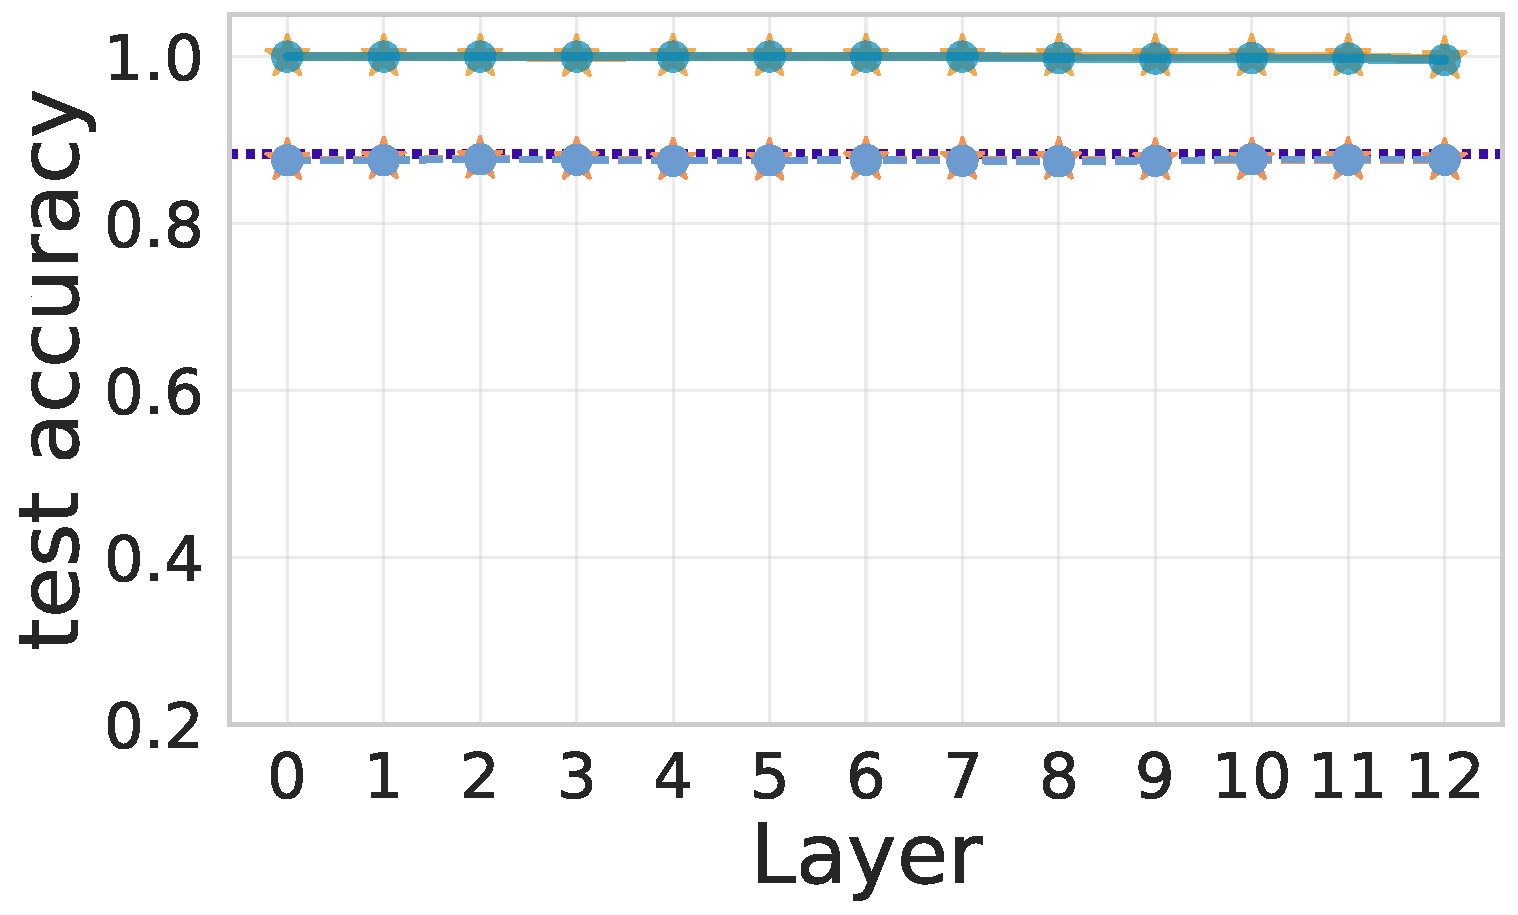
\includegraphics[width=\linewidth]{results_combined/is_aromatic.pdf}
    \subcaption{is aromatic}
    \label{fig:acc-is-aromatic}
\end{subfigure}\hfill
\begin{subfigure}[t]{0.24\textwidth}
    \centering
    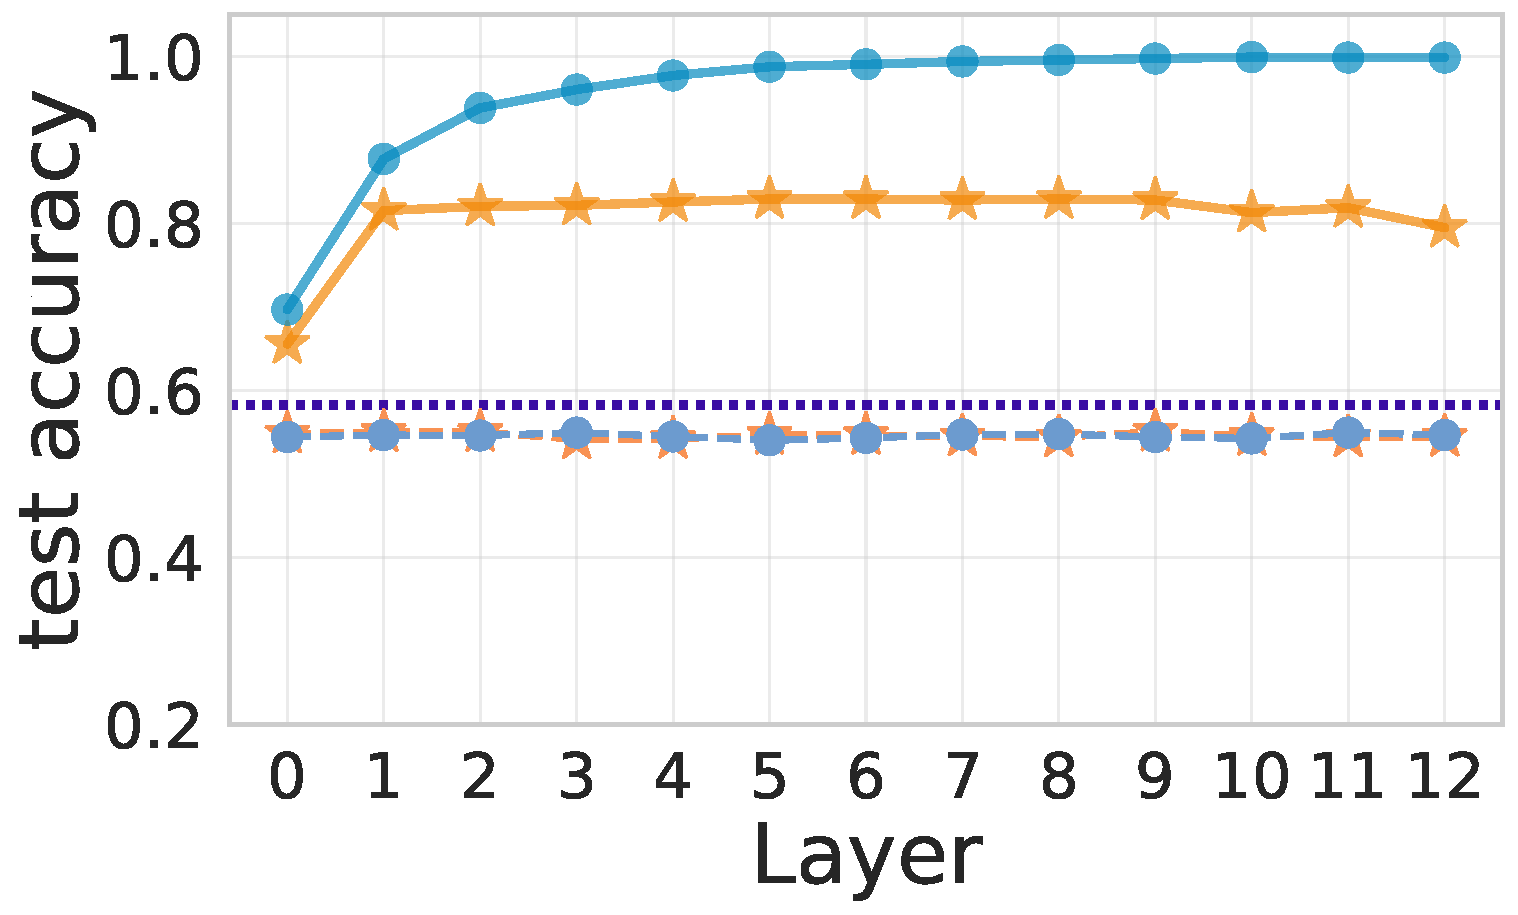
\includegraphics[width=\linewidth]{results_combined/is_in_ring.pdf}
    \subcaption{is in ring}
    \label{fig:acc-is-in-ring}
\end{subfigure}\hfill
\begin{subfigure}[t]{0.24\textwidth}
    \centering
    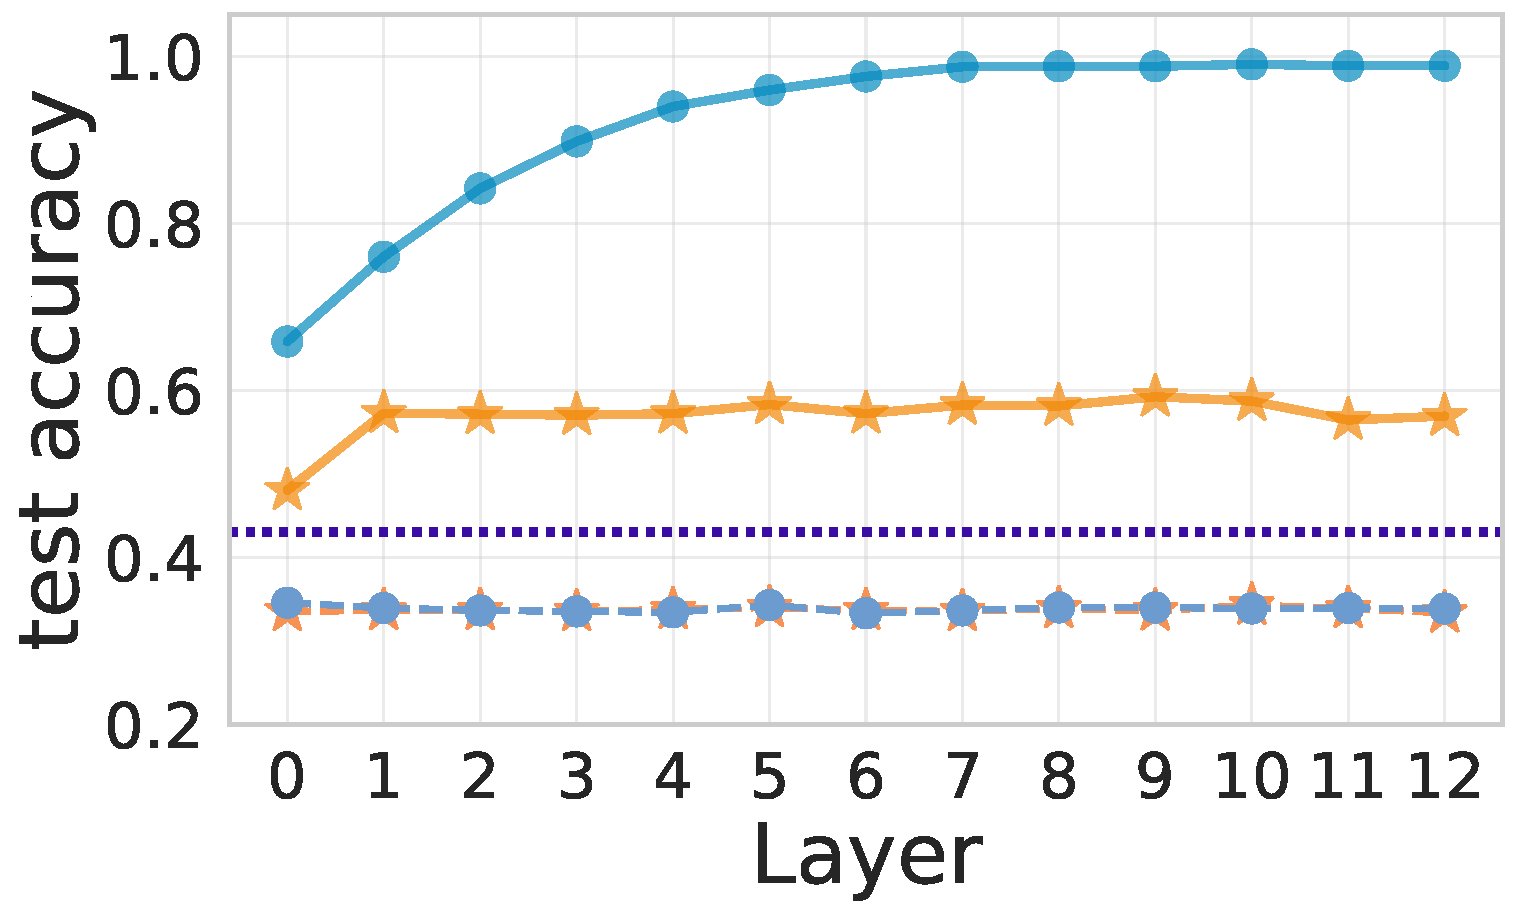
\includegraphics[width=\linewidth]{results_combined/degree.pdf}
    \subcaption{degree}
    \label{fig:acc-degree}
\end{subfigure}\hfill
\begin{subfigure}[t]{0.24\textwidth}
    \centering
    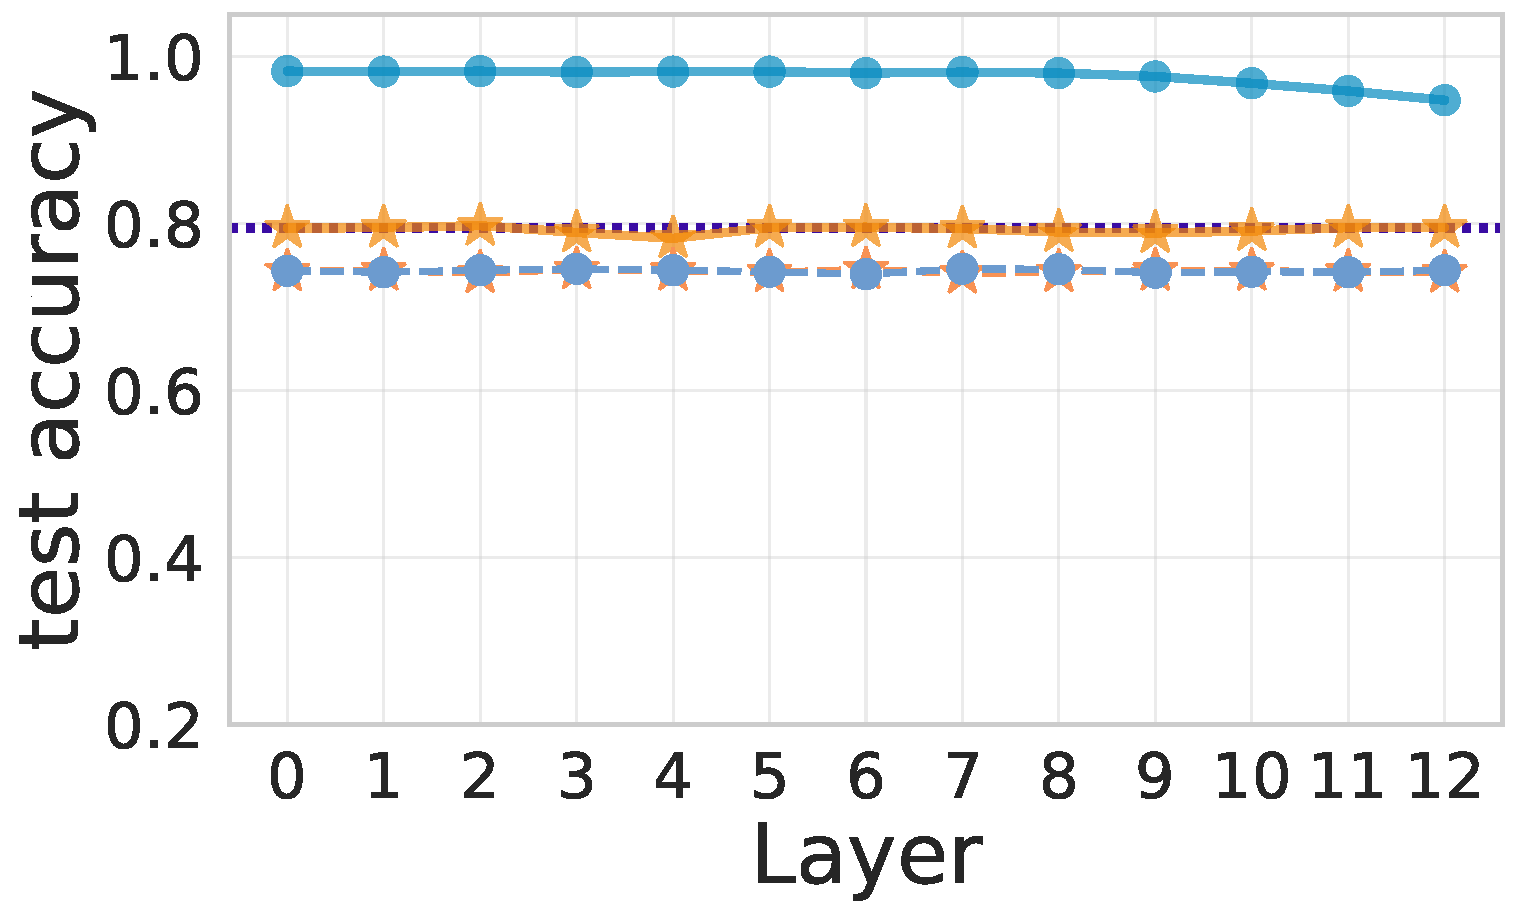
\includegraphics[width=\linewidth]{results_combined/chiral_tag.pdf}
    \subcaption{chiral tag}
    \label{fig:acc-chiral-tag}
\end{subfigure}

\vspace{0.4em}

\begin{subfigure}[t]{0.24\textwidth}
    \centering
    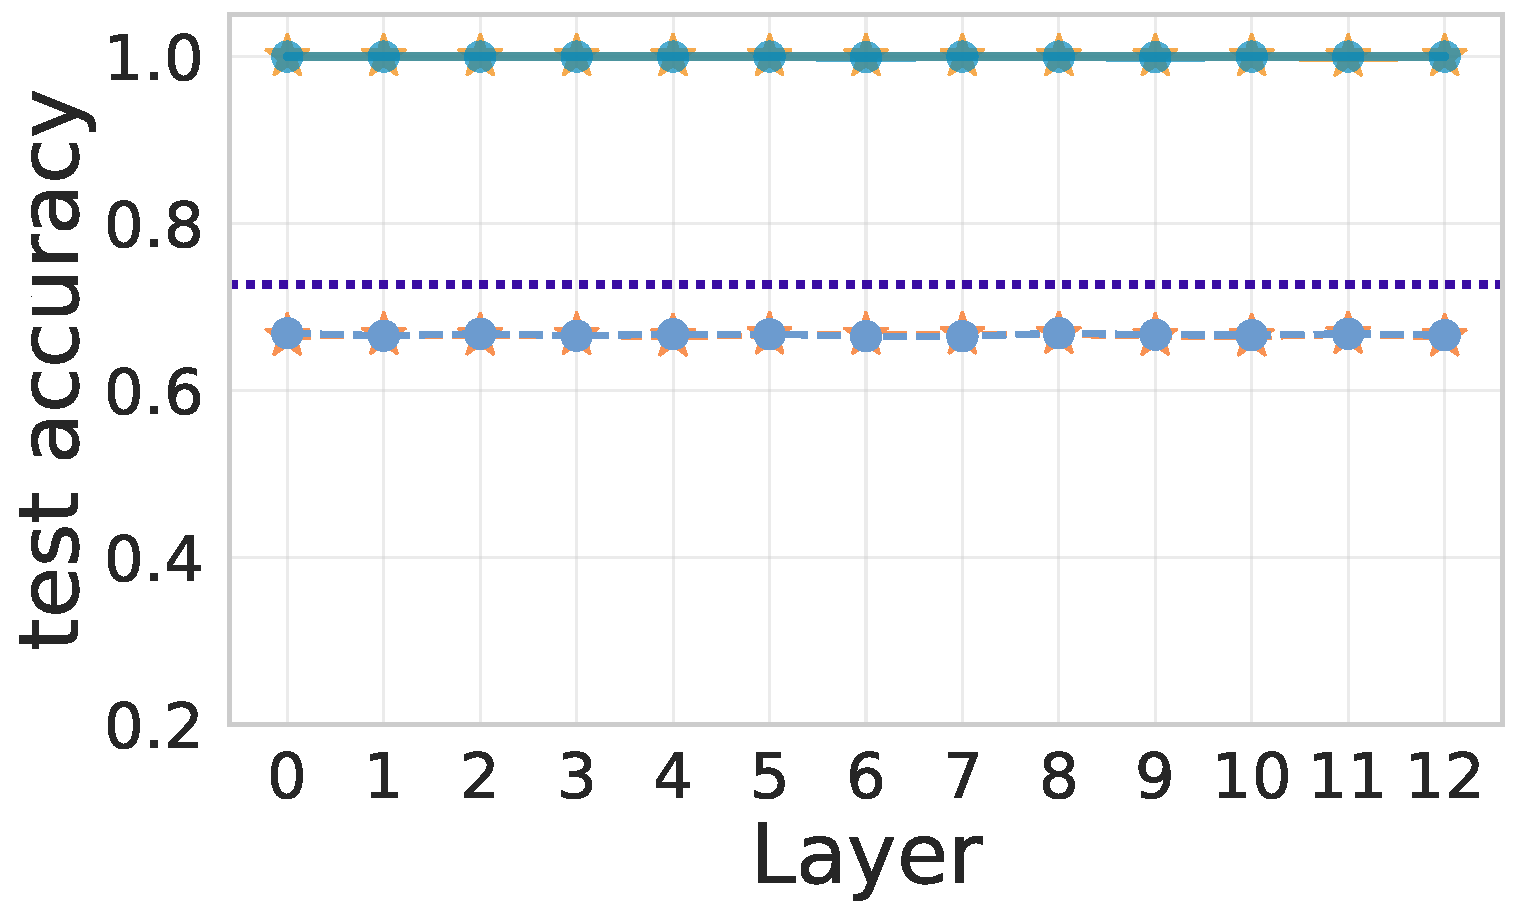
\includegraphics[width=\linewidth]{results_combined/atom_type.pdf}
    \subcaption{atom type}
    \label{fig:acc-atom-type}
\end{subfigure}\hfill
\begin{subfigure}[t]{0.24\textwidth}
    \centering
    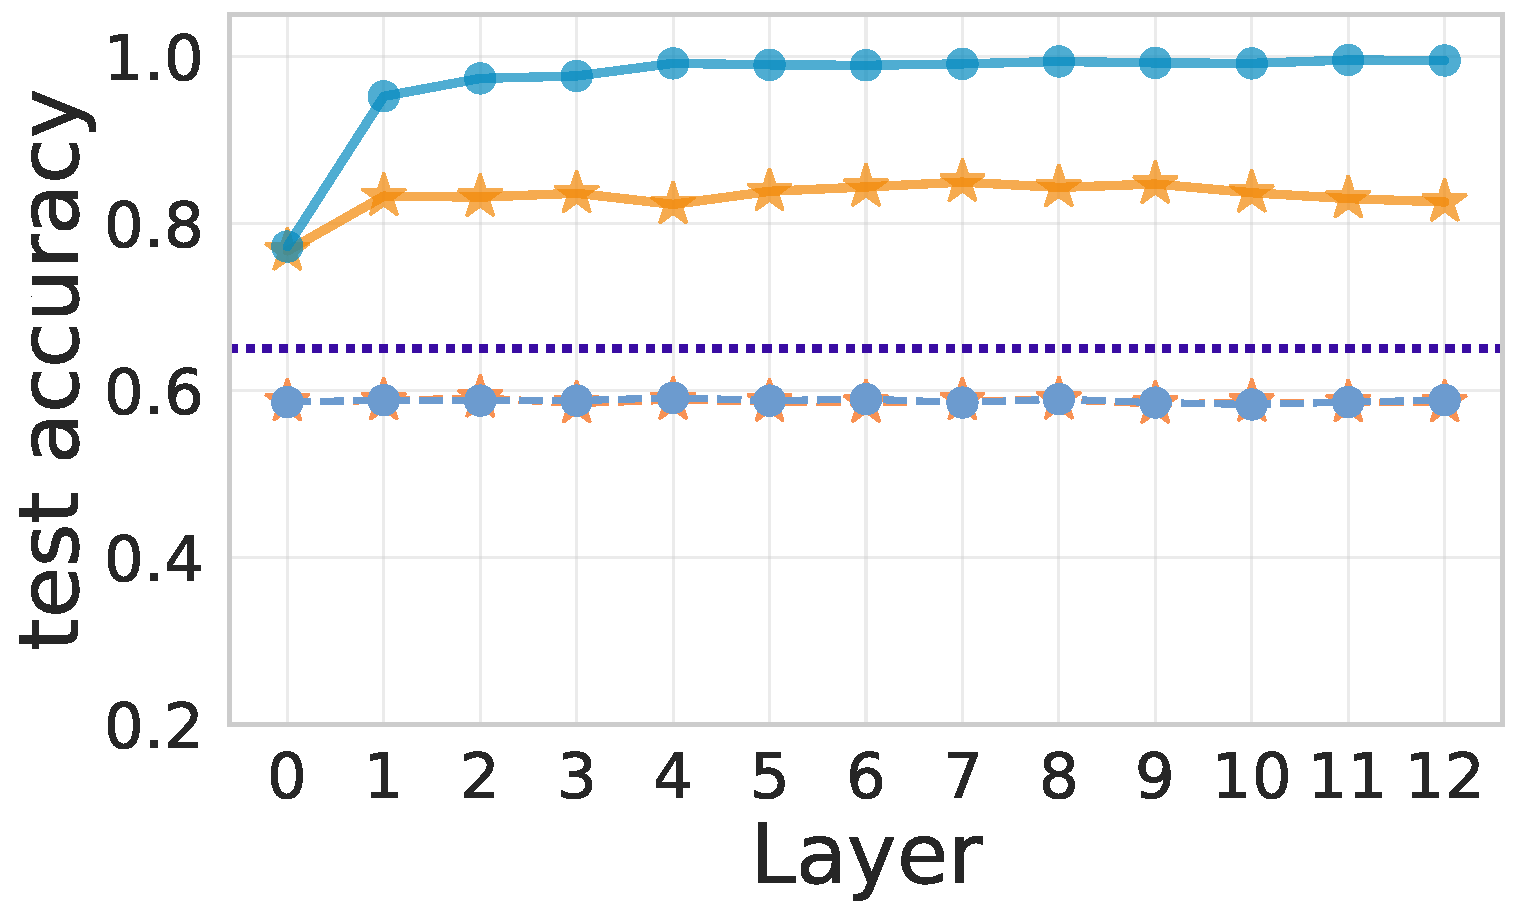
\includegraphics[width=\linewidth]{results_combined/hybridization.pdf}
    \subcaption{hybridization}
    \label{fig:acc-hybridization}
\end{subfigure}\hfill
\begin{subfigure}[t]{0.24\textwidth}
    \centering
    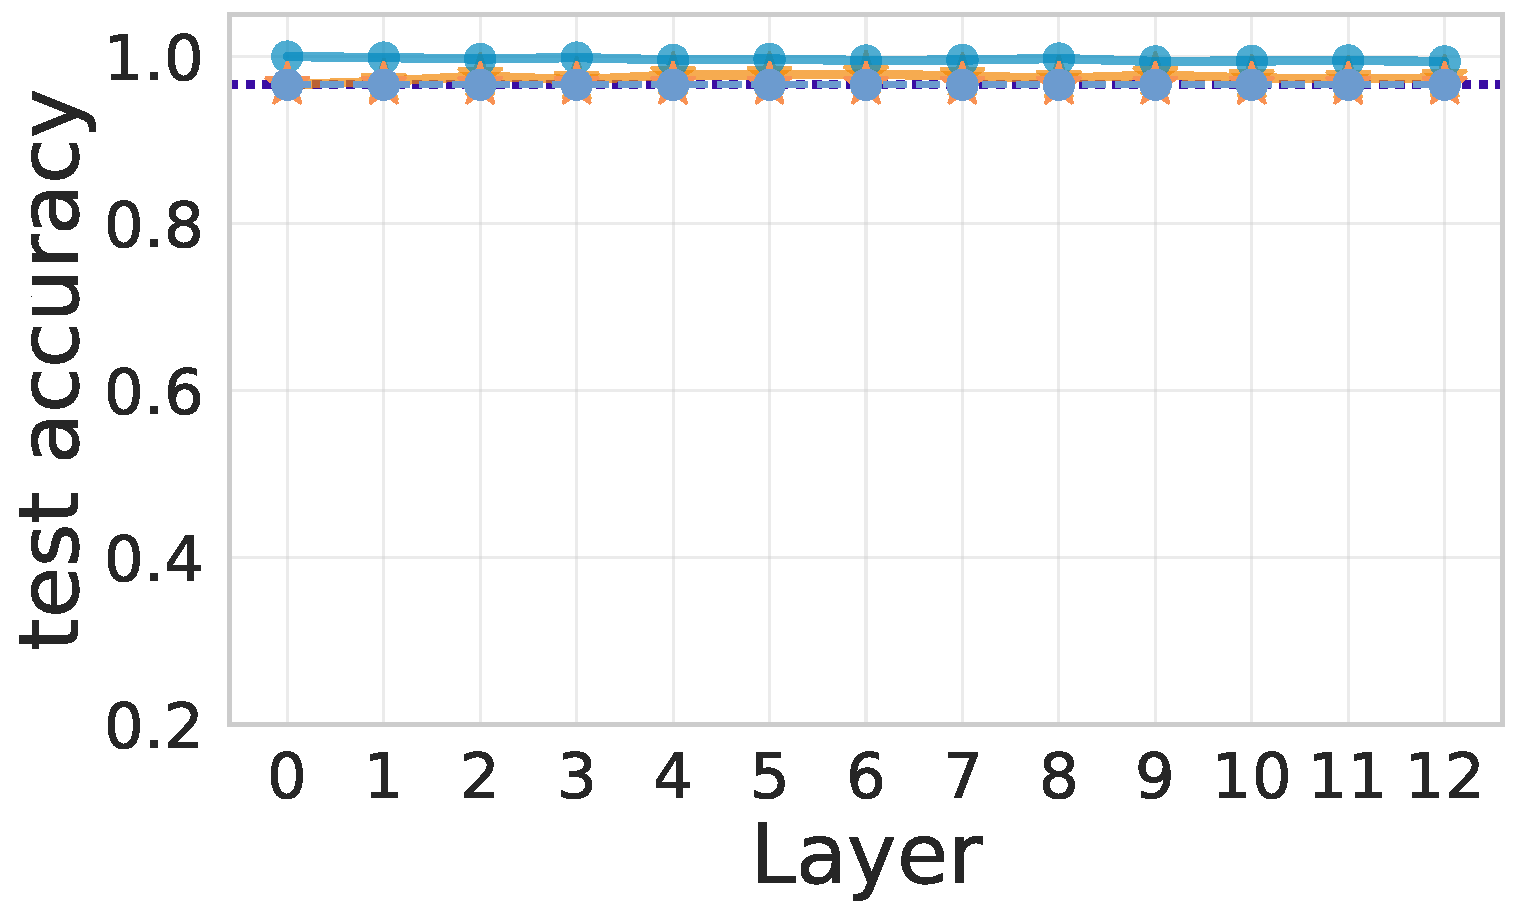
\includegraphics[width=\linewidth]{results_combined/formal_charge.pdf}
    \subcaption{formal charge}
    \label{fig:acc-formal-charge}
\end{subfigure}\hfill
\begin{subfigure}[t]{0.24\textwidth}
    \centering
    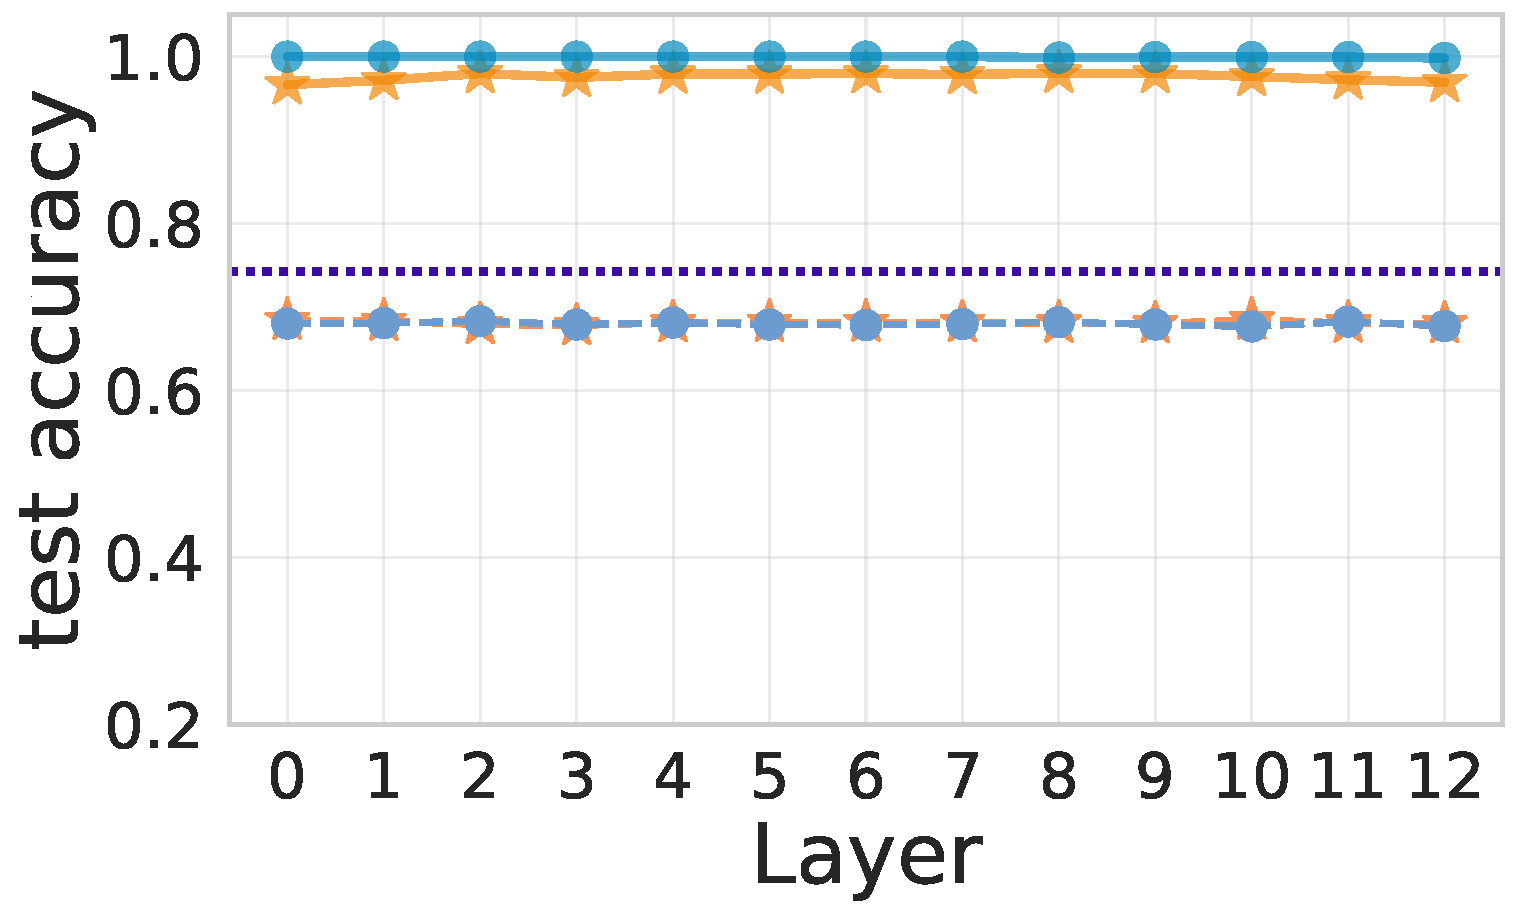
\includegraphics[width=\linewidth]{results_combined/total_valence.pdf}
    \subcaption{total valence}
    \label{fig:acc-total-valence}
\end{subfigure}

\vspace{0.4em}

\centerline{
\includegraphics[width=0.9\textwidth]{results_combined/legend.pdf}}

\caption{Linear-probe test accuracy per layer on eight per-atom QM9 properties. \smi reaches near-perfect accuracy by mid-layers on the contextual properties (ring membership, degree, chiral tag, hybridization, total valence), while \molm plateaus several points below; the surface-form properties (atom type, aromaticity) saturate at the embedding in both models.}
\label{fig:acc}
\end{figure*}
